\section{Design and Implementation}

\kwa{(The unused Listing 3.3 is removed.)}


 This section describes the design and implementation of PyTorch-Direct.
First, we provide an overview of design goals and introduce a new type of tensor, i.e., \textit{the unified tensor}, which incorporates new concepts in need.
We then discuss the unified tensor API and its advanced configurations.
Finally, we describe our implementation and optimizations.

\subsection{Overview}
\label{sec.PyTorch_direct.Overview}


PyTorch-Direct aims to enable GPU out-of-memory training and inference for GNN while incorporating the direct access feature to improve data access performance.
To achieve this, PyTorch-Direct presents to the developers several API features centered around a new type of tensor called ``unified tensor''.
It is a new, independent type parallel to PyTorch native GPU or CPU tensors from both the user interface perspective and its implementation in the runtime system. We have developed all the supporting code that allows unified tensors to be used as a full-fledged tensor type in all PyTorch runtime activities such as memory allocator, \texttt{torch.device} class, dispatch, etc. This makes it extremely easy for the application developers to adapt their PyTorch code to use unified tensors.


 
Unified tensors are at the core of the PyTorch-Direct design, which enables GPUs to directly operate on the host memory.
\kwc{All} CUDA and CPU C++ \kwc{kernels in} PyTorch runtime can directly access unified tensors by simply dereferencing their memory pointers.
In comparison, PyTorch native CPU tensors can only be accessed by CPU, and CUDA tensors can only be accessed by GPU, thus limiting the type of computation devices that can participate in processing these tensors.
Unified tensors eliminate these limitations.
\hide{\hl{Compute-oriented, not data oriented}}

By default, PyTorch-Direct allocates the unified tensors in the host memory and allows GPUs to directly access them over the PCIe.
Since the unified tensors are located in the host memory, their sizes can grow beyond the GPU memory size.
From the CPU's perspective, accessing the unified tensors is identical to accessing CPU tensors.

\begin{lstlisting}[label=unified-example-original,caption=An example of GNN training in PyTorch.,frame=tb,float=]
 # Load features into regular CPU tensor
 features = dataload()
  
 for epoch in range(num_epochs):
   for (neighbor_id, <@\ldots@>) \
     in enumerate(neighbor_sampler):
      
     # Gather features using neighbor_id
     # and then copy to GPU
     input_features = \
       features[neighbor_id].to("cuda")
          
     train(input_features, <@\ldots@>)<@\lstsetnumber{\ldots}@>
     <@\ldots@><@\lstsetnumber{}@><@\lstresetnumber\setcounter{lstnumber}{299}@>

\end{lstlisting}




Application developers can adapt their PyTorch code to use unified tensors with minimal changes to their code.
In Listing \ref{unified-example-original}, we show a simplified example of GNN training in PyTorch.
After loading all the features into host memory, in every training step, it sends the features in the mini-batch to the GPU by calling \texttt{to("cuda")} before invoking the \texttt{train} function (lines 10--13).


The procedure with the unified \kwc{tensor} is shown in Listing \ref{unified-example}.
In this example, to migrate to the unified tensor scheme, the developer only needs to remove the \texttt{to("cuda")} invocation on \texttt{features[neighbor\_id]} and instead invoke \texttt{to("unified")} on \texttt{features} at the beginning.
The features of the whole graph are now stored in a unified tensor that can hold data beyond the GPU memory capacity.
After that, GPU kernels that are launched by the \texttt{train()} function can directly access \texttt{features} since it can access \kwc{a} unified tensor and its derived tensors.
Therefore, \texttt{to()} \kwc{calls are} not needed anymore.
Section \ref{sec.PyTorch_direct.API} describes more about the API design, including advanced configurations.



\kwc{As a full-fledged tensor type,} unified tensor \kwc{facilitates} a clean implementation of complicated rules in runtime systems and easy future extensions.
For example, PyTorch-Direct clearly defines the whole set of rules to resolve computation placement and output tensor placement for computation that involves unified tensors, as detailed in Section \ref{sec:placement_rules}. Thanks to the completeness of the unified tensor, this \kwc{ruleset} is well integrated into the PyTorch runtime system. The implementation details are discussed in Section \ref{sec:impl},

\begin{lstlisting}[label=unified-example,caption=GNN training in PyTorch-Direct with unified tensor. Only two lines (2 and 11) from Listing \ref{unified-example-original} are changed to incorporate unified tensor., frame=tb,float=]
 # Load features into unified tensor
 features = dataload().to("unified")
  
 for epoch in range(num_epochs):
   for (neighbor_id, <@\ldots@>) \
     in enumerate(neighbor_sampler):
      
     # GPU directly fetches required
     # features from unified tensor
     input_features = \
       features[neighbor_id]
          
     train(input_features, <@\ldots@>)<@\lstsetnumber{\ldots}@>
     <@\ldots@><@\lstsetnumber{}@><@\lstresetnumber\setcounter{lstnumber}{299}@>
\end{lstlisting}

\subsection{API Design}
\label{sec.PyTorch_direct.API}

\begin{table}[]
\centering
\begin{tabular}{ll}
\toprule
Example                           & Description                                                                                      \\\midrule
\texttt{t.to("unified")}                   & \begin{tabular}[c]{@{}l@{}}Copy the tensor \texttt{t} to unified\\  device.\end{tabular}                   \\
\texttt{torch.ones(16, device="unified")} & \begin{tabular}[c]{@{}l@{}}Specify unified device in \\ PyTorch native APIs.\end{tabular}        \\
\texttt{t.is\_unified}                     & \begin{tabular}[c]{@{}l@{}}Return true if the tensor \texttt{t} \\ is a unified tensor.\end{tabular}      \\
\texttt{unified\_tensor + cpu\_tensor}       & \begin{tabular}[c]{@{}l@{}}Compute with hybrid tensors \\ of unified and CPU types.\end{tabular} \\
\texttt{unified\_tensor[gpu\_tensor]}   & \begin{tabular}[c]{@{}l@{}}Subscript unified tensor with \\  CUDA tensor.\end{tabular}     \\
\bottomrule
\end{tabular}
    \caption{Typical usage of APIs with unified tensor. Unified tensors are allowed for easy creation and flexible computation.}
    \label{tab:APIUnified}
\end{table}

PyTorch-Direct APIs are designed to provide an interface to unified tensors in the idiomatic PyTorch manner.
Table \ref{tab:APIUnified} demonstrates the typical use of unified tensor APIs.
Developers can create a unified tensor by copying from another tensor via PyTorch built-in \texttt{to()} method of \texttt{torch.Tensor}.
It can also be created from scratch by specifying the \texttt{device} argument as the unified device in PyTorch APIs, such as \texttt{torch.ones}.
The user can check if a tensor is of unified type by \kwc{checking} the \texttt{is\_unified} \kwc{attribute}.

Unified tensors can be computed with CPU or CUDA tensors, providing great flexibility.
Meanwhile, they are free from redundant data movements since the CPU and GPU can directly access their underlying memory without creating temporary copies.
By contrast, in the native PyTorch API, CPU tensors typically cannot work with CUDA tensors because of the device binding unless additional routines to handle them have been implemented in the PyTorch runtime system.
For example, the subscript operator allows a CUDA tensor to be indexed by a CPU tensor, and binary and comparison operators accept GPU scalar and CPU scalar as the two operands.


\subsection{Computation and Storage Placements}
\label{sec:placement_rules}
\begin{table}[!htbp]
\begin{subtable}[]{\textwidth}\centering
\begin{tabular}{lll}
\toprule
\multicolumn{3}{c}{All unified tensors are GPU-affinitive.}        \\
\midrule
\multirow{2}{6.2cm}{No less than one operand is non-scalar CPU tensor.}   & \multicolumn{1}{l|}{compute on} & GPU  \\
 & \multicolumn{1}{l|}{output type}& host-affinitive unified \\
\hline
\multirow{2}{6.2cm}{Previous row is false. And no less than one operand is CUDA type.}  & \multicolumn{1}{l|}{compute on} & GPU  \\%\cline{2-4} 
 & \multicolumn{1}{l|}{output type}& GPU   \\
\hline
\multirow{2}{6.2cm}{Operands are either unified tensors or CPU scalars.}   & \multicolumn{1}{l|}{compute on} & GPU  \\%\cline{2-4} 
 & \multicolumn{1}{l|}{output type} & GPU   \\
\bottomrule
\vspace{0.05em}
\end{tabular}
\end{subtable}

\begin{subtable}[]{\textwidth}\centering
\begin{tabular}{lll}
\toprule
\multicolumn{3}{c}{At least one unified tensor is host-affinitive.}      \\
\midrule
\multirow{2}{5cm}{No less than one operand is non-scalar CPU tensor.}   & \multicolumn{1}{l|}{compute on}  & \begin{tabular}[c]{@{}l@{}}CPU if no operand is \\ GPU-affinitive, else GPU\end{tabular} \\
& \multicolumn{1}{l|}{output type} & host-affinitive unified  \\
\hline
\multirow{2}{5cm}{Previous row is false. And, no less than one operand is CUDA tensor.} & \multicolumn{1}{l|}{\multirow{2}{*}{compute on}} & \multirow{2}{*}{GPU}\\
& \multicolumn{1}{l|}{}                            &  \\
& \multicolumn{1}{l|}{output type}                 & host-affinitive unified     \\
\hline
\multirow{2}{5cm}{Operands are either unified tensors or CPU scalars.}   & \multicolumn{1}{l|}{compute on}  & \begin{tabular}[c]{@{}l@{}}CPU if no operand is \\ GPU-affinitive, else GPU\end{tabular} \\
& \multicolumn{1}{l|}{output type} & host-affinitive unified  \\
\bottomrule
\end{tabular}
\end{subtable}
\caption{Rules of placements for operators involving unified tensors as operands.}
\label{tab:place_rule}
\end{table}
Though unified tensors can be accessed by both CPU and GPUs, \kwc{we need to define} scheme to determine the computation device and the location of result tensors.
Especially, this \kwc{scheme} may be \kwc{complicated} in scenarios where the operator involves more than two tensors or a hybrid of native tensors and unified tensors.

In the original PyTorch, the dispatch mechanism determines the computation device and result tensor type based on input tensor metadata before executing the operator.
We followed the same idea and integrated a set of lightweight rules into the existing dispatch mechanism.
This allows it to be better integrated into the PyTorch runtime and leads to low overhead in performance and programmer effort to adopt the unified tensor.
There might be more sophisticated ideas, such as computational graphs, but they may drastically change the APIs or cause a bigger performance overhead.

Each unified tensor is designated an affinity mode, either host-affinity or GPU-affinity.
In the simplest scenario where an operator is applied to a unified tensor in host-affinity mode, the computation and results tensors are placed on the host during execution.
Similarly, if this happens to a unified tensor in GPU-affinity mode, the computation and result are placed on the GPU.
The reasoning behind the two modes is simple.
In GNN mini-batch input transfer, we want the results to stay on the GPU as they are consumed by kernels executing the GNN on the GPU, thus avoiding unnecessary data transfers over PCIe.
Therefore, the output tensor should be of CUDA type.
This is what the GPU-affinity mode is for.
On the other hand, the host-affinity mode allows the result tensor to stick to the unified tensor type and allows for more preprocessing.
One can switch \kwc{a host-affinitive unified tensor} to GPU-affinity mode once the preprocessing is done.

Switching the affinity mode of a unified tensor can be done easily by a new tensor method.
It does not incur movements.

Table~\ref{tab:place_rule} shows the complete set of rules.
The number of scalar CPU tensors influences the placement to stay consistent with the existing PyTorch dispatch logic.
The other factor is if CUDA tensors are participating in the operator because, in that case, the only feasible computation devices are GPUs.




\subsection{Implementation}
\label{sec:impl}
While offering seamless API integration into the existing PyTorch design, this project also integrates it into the PyTorch runtime C++ code in a neat, modular, and extensible way.

The goal of implementation is to realize the flexibility and performance benefits of the unified tensor while keeping modifications to existing logic as minimal as possible, especially with the large number of operator definitions.


The core object in the PyTorch runtime system is \texttt{at::Tensor}.
Every PyTorch tensor (\texttt{torch.Tensor} object) is a \texttt{THPVariable}\footnote{\kwc{``\texttt{THP}'' stands for TorcH Python}~\cite{edwardz.yangPytorchTorchCsrc2017}.} object in C++ runtime code, which is the wrapper class combining an \texttt{at::Tensor} object with Python metadata.
The PyTorch runtime dispatches each method call to the proper definition according to the device and data types of the tensor arguments.
A PyTorch method operating on tensors eventually goes into a function of \texttt{at::Tensor}\footnote{\kwc{``at'' stands for the ``A TENsor'' library}~\cite{edwardz.yangATenAtenSrc2018}.}.


PyTorch-Direct implements the unified tensor mechanisms in the PyTorch runtime as a complete type of tensor.
This makes the design modular, extensible, and well-integrated into the PyTorch runtime code.
A new memory allocator is implemented to govern the memory allocation for all unified tensors.
It adapts the allocation \kwc{pool} mechanism from the PyTorch CUDA allocator to reduce the number of CUDA API invocations.

Two dispatch keys are added, corresponding to the two affinity modes mentioned in Section~\ref{sec:placement_rules}.
Dispatch keys specified by each tensor inform the dispatcher to dispatch the operator to the correct backend to get executed.
The introduced zero-copy memory allocator uses PyTorch's pooling idea in PyTorch's original CUDA to reduce API invocations.
Besides, auxiliary logic in the build system and runtime is modified to incorporate the changes.
Only the device-checking logic needs to be changed for most operator definitions, as it now needs to recognize the new unified tensor type.

This project is first developed on top of PyTorch 1.6.
Around 2.6K lines of code are added or modified to incorporate the complete mechanism detailed in this section.
To support the latest CUDA microarchitecture in Section~\ref{sec:pytorch_direct_evaluation}, we then migrated the minimal functional part to nightly PyTorch 1.8.


\subsection{Memory Alignment Optimization}
\label{sec.PyTorch_direct.implementation.alignment}


To achieve efficient PCIe data transfer, memory requests from the GPU threads in the same warp should be aligned and merged to the GPU cacheline (128-byte) granularity~\cite{minEMOGIEfficientMemoryaccess2020}.
However, the default PyTorch GPU indexing function does not guarantee memory alignment unless the input feature tensors are naturally aligned with the GPU cacheline size.
In Figure~\ref{fig:alignment_problem}, we depict a simplified working mechanism of the default PyTorch GPU indexing function.
In this specific example, we scale down the warp size (32 threads in real) and the GPU cacheline size (128 bytes in real) by a factor of eight.
We assume each feature is 4 bytes, and each node has 11 features.
Now, due to the size mismatch between the cacheline (16-byte) and the node feature (44-byte), misaligned accesses can occur.


In the example of Figure~\ref{fig:alignment_problem}, assume that the GPU needs to access nodes 0, 2, and 4.
To achieve this, each thread accesses a single feature.
For example, the first 11 threads access the 11 features of node 0; the following 11 threads access the 11 features of node 2, and so on.
This looks simple in a logical view on the left side of Figure~\ref{fig:alignment_problem}, where we highlight the accesses of threads 11--21 to features of node 2.
However, when we redraw the access patterns based on cacheline and warp alignments on the right side of Figure~\ref{fig:alignment_problem}, we see that the accesses are fragmented into multiple cachelines and warps.

To solve the problem of misaligned access patterns, we use a circular shift method as described in Figure~\ref{fig:alignment_fix}.
In this method, all threads calculate the required index offset values to make aligned accesses.
In the case of Figure~\ref{fig:alignment_fix}, the threads need to do a right shift by an offset of one.
The threads on the edges check the boundary conditions and make additional adjustments by adding or subtracting the length of the node feature so that they do not accidentally access the other node features.
When the indexed values are written to the output, the output indices are also identically adjusted to maintain the ordering.
With the optimization, PyTorch-Direct reduces the number of total PCIe requests from seven to five in this case.
Inside the PyTorch GPU indexing kernel, we check the input tensors and apply this optimization only when the input tensors are unified tensors and the feature widths are not naturally aligned to 128-byte granularity.
All these adjustments are automatically made due to our modifications to PyTorch source code. As such, no programmer effort is required to solve the memory alignment problem.


\begin{figure}[]
    \centering
    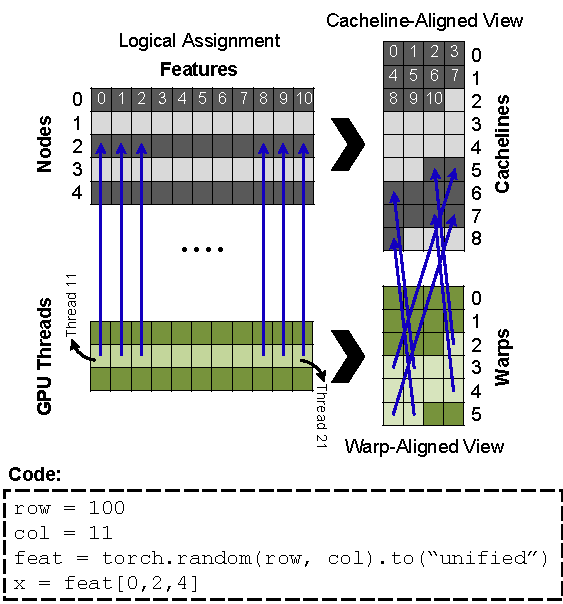
\includegraphics[width=0.7\linewidth]{figures/PyDArXiv/alignment_problem.pdf}
    \caption{Data access misalignment occurring in PyTorch-Direct when using unmodified PyTorch indexing scheme. Based on the code, thread 0--10 access \texttt{feat[0]}, thread 11--21 access \texttt{feat[2]}, and thread 22--32 access \texttt{feat[4]}. For the case accessing \texttt{feat[2]} (blue arrows), we can easily identify the accesses are fragmented into multiple warps and cachelines.}
    \label{fig:alignment_problem}
\end{figure}

\begin{figure}[]
    \centering
    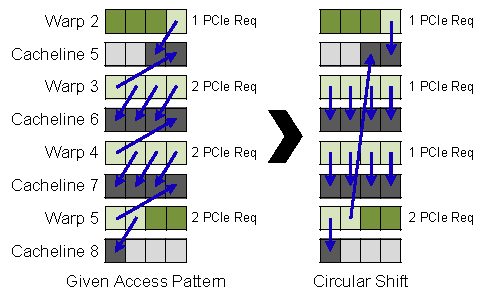
\includegraphics[width=0.7\linewidth]{figures/PyDArXiv/alignment_fix.pdf}
    \caption{Memory alignment optimization with a circular shift. The example is identical to the case in Figure~\ref{fig:alignment_problem}. Alignment reduces the total number of PCIe requests (req) from seven to five in this case.
    }
    \label{fig:alignment_fix}
\end{figure}
